% !TeX root = ../main.tex
\chapter{Score-Informed Transformer Correction for AMT Velocity Estimation}
\label{ch:scoreinf}

\noindent\textbf{Chapter provenance.}
This chapter is adapted from the updated SMC 2026 paper on score-informed MIDI velocity refinement.
The core method, main figures, and principal experimental results are retained.
The main thesis-specific additions are a broader problem framing, explicit retention of an early BiLSTM correction design, and expanded discussion of generalization and robustness.

\section{Chapter Overview and Position in the Thesis}
\label{sec:scoreinf:overview}

This chapter addresses Scenario S2 of the thesis.
In this setting, a performance audio recording and an aligned symbolic score are both available.
This situation is common in music education, rehearsal analysis, and curated audio--score archives.
The score supplies reliable note content and approximate temporal structure.
However, its expressive information is often incomplete, simplified, or unreliable.
At the same time, modern automatic music transcription (AMT) systems can estimate note-level MIDI velocity from audio, but these estimates remain noisy and sensitive to acoustic domain shift.
The central question of this chapter is therefore simple and practical: \emph{when note events are already known from a score, how should score information be used to improve AMT-estimated velocity without redesigning the whole transcription backbone?}

This question is important beyond one benchmark.
Recent progress in velocity-enabled piano AMT has supported the creation of expressive piano corpora and downstream applications such as expressive rendering, music education, and performance-aware generation \cite{amt2019ov,hung2021emopia,kong2022giantMIDI,zhang2022atepp,edwards2023pijama,chou2024midibert,zhang2024dexter,he2025filling}.
Yet the practical availability of note-level dynamics still lags behind the availability of audio and score.
In many real collections, a score exists but its velocity values are either quantized, manually entered, inherited from notation defaults, or simply unrelated to the performed dynamics.
This creates a natural score-informed correction problem rather than a pure end-to-end transcription problem.

From the thesis perspective, the present chapter occupies the middle point of Thread~A.
Chapter~\ref{ch:velcomp} studied symbolic-only recovery when a MIDI representation is present but its velocities are missing.
The present chapter keeps the note-level velocity target but introduces real audio and aligned score support.
Chapter~\ref{ch:audiodyn} will then move toward broader score-level dynamic attributes.
Taken together, these chapters test how expressive information can be recovered under progressively weaker supervision.

A second thesis-level motivation concerns model reuse.
AMT backbones evolve rapidly, from CRNN designs to frequency--time Transformers and event-based models \cite{kong2021hpt,wei2022hppnet,toyama2023hft,yan2024semicrf}.
If each score-informed system requires a new early-fusion architecture, then any gain in velocity estimation is tightly coupled to one backbone generation.
This chapter instead asks whether score information can be injected \emph{late}, as a lightweight correction layer, so that the same idea remains reusable as AMT front ends change.
This design choice is what distinguishes the chapter from earlier score-informed work.

\section{Task-Specific Related Work and Motivation}
\label{sec:scoreinf:related}

Score-informed MIDI velocity estimation developed in parallel with velocity-enabled AMT.
Earlier studies estimated note intensity from piano recordings with hand-crafted acoustic measurements, statistical analysis, or score-informed factorization \cite{dan2006psy,ewert2011est,jeong2017note,jeong2018timbre}.
These studies established the feasibility of the task, but their dependence on manual parameterization limited portability across datasets and recording conditions.
More recent work moved to deep learning and showed that aligned score information can substantially improve note-level dynamics estimation \cite{kim2023score,kim2024method,kim2023diffvel}.
The most competitive of these systems use feature fusion, where score information is injected into the acoustic network during feature extraction.

Those feature-fusion approaches are effective, but they also create a practical bottleneck.
The score-informed mechanism becomes entangled with the acoustic encoder.
As a result, the whole system must usually be re-engineered for each new AMT backbone.
This is awkward in a fast-moving research area where strong transcription front ends already exist and continue to improve.
For a thesis contribution, accuracy alone is not enough.
The method should also expose a reusable principle.
This is the main reason for the late-correction stance adopted in this chapter.

This chapter is also closely related to velocity-enabled piano AMT.
Modern systems such as HPT, HPPNet, hFT-Transformer, and Transkun v2 already estimate MIDI velocity together with note events \cite{kong2021hpt,wei2022hppnet,toyama2023hft,yan2024semicrf}.
However, audio-only velocity estimation remains acoustically fragile.
Recent analysis shows that transcription models can absorb strong sound and recording biases, which then harm cross-dataset behaviour \cite{martak2026soundmusicbias}.
This makes score-informed refinement attractive even when the AMT backbone is already strong.
The role of the aligned score is not to replace audio.
Its role is to provide acoustics-invariant structure that constrains how the audio-driven estimate should be corrected.

Finally, the chapter should be distinguished from audio--score alignment work.
Alignment studies correct \emph{when} a note occurs in the score relative to the audio \cite{morsi2022bottlenecks,zeit2024align,chang2025rumaa}.
The present problem is different.
We assume that note content and note timing are already available through alignment, and we focus on \emph{how strongly} each aligned note was played.
This narrow focus is deliberate.
It lets the chapter isolate note-level dynamics recovery as a standalone problem.

\section{Problem Setting}
\label{sec:scoreinf:problem}

The task studied in this chapter is \emph{score-informed MIDI velocity estimation}.
Given a piano performance audio recording and a time-aligned score, we seek to output MIDI notes with corrected note-level velocity values.
The score is assumed to provide the note events that should receive a velocity value.
The remaining problem is the estimation or correction of velocity at each note onset.

This setting is practically important for two common use cases.
First, educational scenarios often provide a reference score together with student performance audio.
Second, large online archives often provide aligned audio--score pairs but do not provide trustworthy expressive labels.
In both cases, an audio-only AMT system leaves dynamics analysis incomplete.
A score-informed system can use symbolic structure to stabilize the estimate while retaining acoustic evidence from the performed sound.

Two assumptions should be stated clearly.
First, the method is designed to correct velocity, not to determine whether a note exists.
Second, the score alignment is assumed to be sufficiently reliable to define note events.
This does not mean the score must be perfectly aligned.
Indeed, later sections explicitly test robustness under moderate artificial timing shifts.
However, the problem formulation still presumes that the score and audio refer to the same performed notes.

Relative to the rest of the thesis, this chapter therefore sits between symbolic completion and higher-level dynamic analysis.
Unlike Chapter~\ref{ch:velcomp}, it operates on real audio and must cope with acoustically induced error.
Unlike Chapter~\ref{ch:audiodyn}, its output remains note-level MIDI velocity rather than broader dynamic categories or change patterns.
This middle position makes it a useful bridge in the thesis narrative.

\section{Modular Correction Principle}
\label{sec:scoreinf:principle}

Previous score-informed approaches typically inject score information during acoustic feature processing.
This early-fusion strategy can work well.
However, it ties the score-informed design to a specific acoustic architecture.
For the thesis objective, a late-correction design is more attractive.
It preserves compatibility with existing AMT pipelines.
It isolates the dynamics refinement problem from note transcription.
It also makes cross-backbone evaluation straightforward.
Figure~\ref{fig:scoreinf_compare} illustrates this distinction.

\begin{figure}[t]
\centering
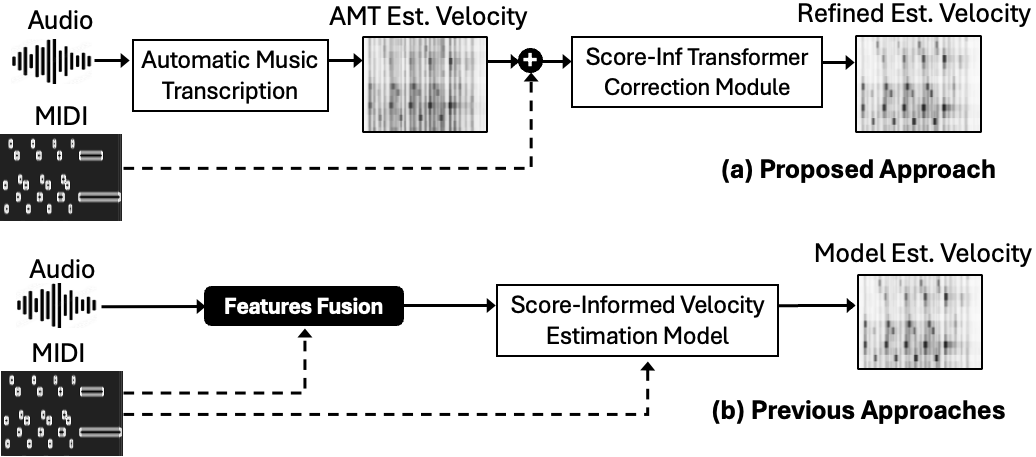
\includegraphics[width=0.8\textwidth]{Chapter_4/figures/p1thesis.jpg}
\caption{Conceptual comparison between the proposed modular correction approach and earlier score-informed feature-fusion approaches.}
\label{fig:scoreinf_compare}
\end{figure}

The interface of the proposed system is intentionally simple.
The AMT backbone first predicts a preliminary velocity map from audio.
The aligned score is then converted into symbolic features at the same time resolution.
A lightweight score-informed module finally corrects the preliminary estimate at note onsets.
This design has three practical advantages.
First, it keeps the acoustic front end reusable.
Second, it allows the correction module to be attached to several AMT backbones with only small engineering changes.
Third, it constrains the score-informed stage to a narrow task.
The module adjusts \emph{how loudly} a note is played.
It does not decide \emph{whether} the note exists.

This separation of roles is important.
The acoustic branch still provides the initial evidence for performance intensity.
The score does not overwrite that evidence.
Instead, it regularizes the estimate by telling the model where notes occur and how they are organized in time.
Later results will show that this division of labour is strong enough to improve both in-domain accuracy and cross-dataset behaviour.

\section{Score-Informed Correction Module}
\label{sec:scoreinf:method}

Figure~\ref{fig:scoreinf_framework} shows the complete framework.
The score-informed module is attached after the velocity branch of a chosen AMT system.
Only the velocity estimate is corrected.
The rest of the transcription backbone remains unchanged.

\begin{figure}[t]
\centering
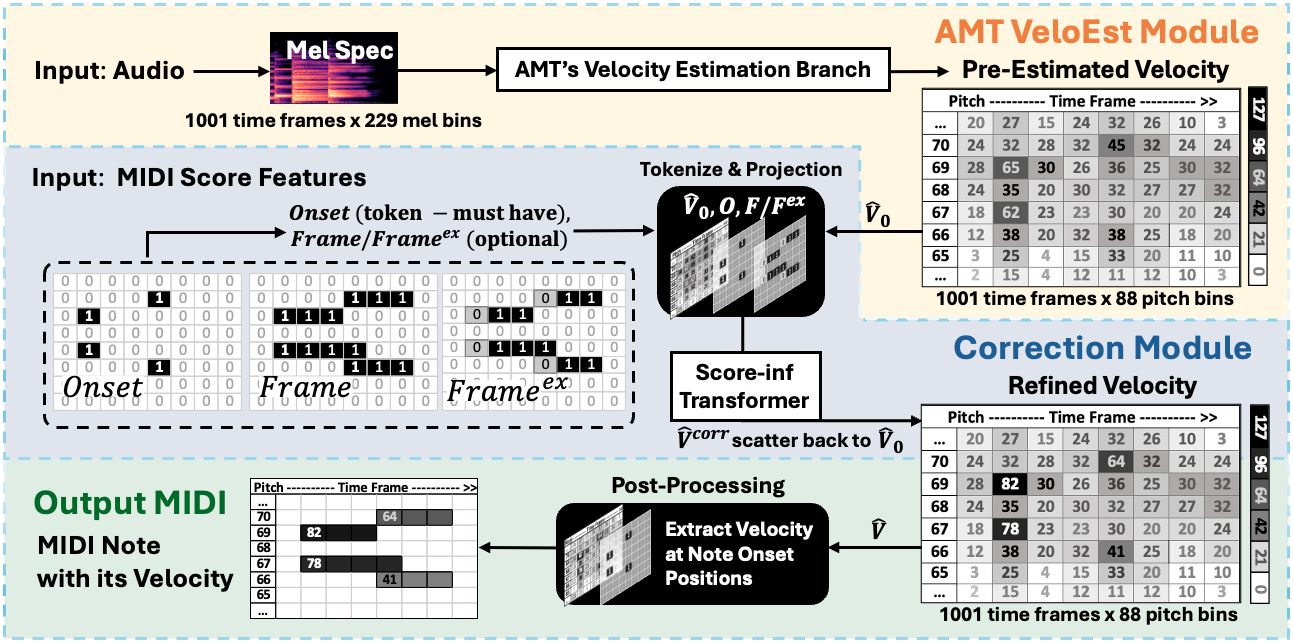
\includegraphics[width=\textwidth]{Chapter_4/figures/p2.jpg}
\caption{Proposed score-informed MIDI velocity estimation framework. The AMT backbone provides a preliminary velocity estimate. The score-informed module refines this estimate using features extracted from the aligned MIDI score.}
\label{fig:scoreinf_framework}
\end{figure}

\subsection{MIDI score features}
\label{sec:scoreinf:features}

Consistent with the standard paradigm of score-informed MIDI velocity estimation \cite{kim2024method}, we rasterize the aligned score into pianoroll-like binary matrices at the same time resolution as the AMT output.
Let $T$ be the number of frames and $P$ the number of piano keys.
In our setting, $T=1001$ and $P=88$.
We define the onset matrix $\mathbf{O}\in\{0,1\}^{T\times P}$, the frame matrix $\mathbf{F}\in\{0,1\}^{T\times P}$, and the onset-excluded sustain matrix $\mathbf{F}^{\mathrm{ex}}\in\{0,1\}^{T\times P}$ as
\begin{equation}
\mathbf{F}^{\mathrm{ex}} = \mathbf{F} - \mathbf{O}.
\label{eq:scoreinf:fex}
\end{equation}
We further define the nonzero index sets
\begin{equation}
\mathcal{I} = \{(t,p)\mid O_{t,p}=1\},
\qquad
\mathcal{J} = \{(t,p)\mid F_{t,p}=1\}.
\label{eq:scoreinf:index}
\end{equation}
The onset set $\mathcal{I}$ is used for tokenization in the Transformer correction module.
The frame set $\mathcal{J}$ is used for loss masking.

\subsection{Architecture}
\label{sec:scoreinf:arch}

The proposed architecture adopts a modular design.
AMT systems are usually multi-task models that estimate onset, offset, frame, and velocity simultaneously.
We isolate the velocity estimation branch of the chosen AMT baseline and extend it with a score-informed correction module.
To make the design choice explicit, we study two correction modules: an early frame-wise BiLSTM retained for ablation, and a token-based Transformer used in the final system.

\textbf{Velocity estimation branch in AMT.}
This component is identical to the velocity branches of the selected AMT baselines, namely HPT~\cite{kong2021hpt}, HPPNet~\cite{wei2022hppnet}, and DynEst~\cite{he2026dynest}.
All settings follow the original implementations and public repositories.
For a fair comparison, all baselines use the same log-Mel spectrogram input with a 22.05~kHz sampling rate, 2048-point FFT, 100~FPS, Hann window, and 229 mel bins.
This yields an input tensor of size $1001\times229$.
The velocity branch outputs a preliminary velocity map $\hat{\mathbf{V}}_0\in[0,1]^{T\times P}$.

\begin{figure}[t]
\centering
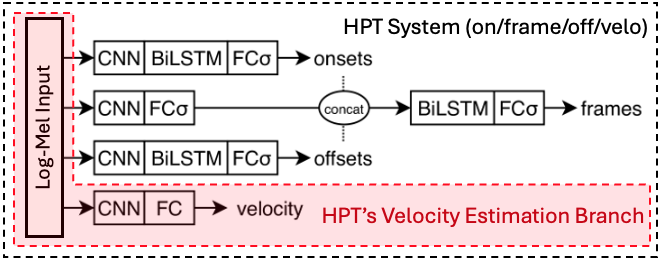
\includegraphics[width=0.85\textwidth]{Chapter_4/figures/p3v1.jpg}
\caption{Velocity Estimation Branch in High resolution piano transcription (HPT) system \cite{kong2021hpt}.}
\label{fig:veloest_branch}
\end{figure}

\textbf{Early design: score-informed BiLSTM correction module.}
As an early design, we first explored a frame-wise bidirectional LSTM (BiLSTM) as the correction module.
At each frame $t$, the preliminary velocity estimate is concatenated with aligned score features along the feature dimension:
\begin{equation}
\mathbf{z}_t =
\left[\hat{\mathbf{V}}_{0,t,:};\, \mathbf{O}_{t,:};\, \mathbf{F}_{t,:}\right]
\quad \text{or} \quad
\mathbf{z}_t =
\left[\hat{\mathbf{V}}_{0,t,:};\, \mathbf{O}_{t,:};\, \mathbf{F}^{\mathrm{ex}}_{t,:}\right],
\label{eq:scoreinf:bilstm}
\end{equation}
where $\mathbf{z}_t\in\mathbb{R}^{3P}$.
The sequence $\{\mathbf{z}_t\}_{t=1}^{T}$ is processed by a BiLSTM with 256 hidden units in each direction, which yields hidden states $\mathbf{h}_t\in\mathbb{R}^{512}$.
A fully connected layer with Sigmoid activation then maps each $\mathbf{h}_t$ to a refined velocity vector $\hat{\mathbf{V}}^{\mathrm{corr}}_{t,:}\in[0,1]^P$.
This variant uses the same score information as the Transformer module, but operates on the full frame sequence rather than onset tokens.
We retain it because it provides a strong and intuitive recurrent baseline for analysis.

\textbf{Final design: score-informed Transformer correction module.}
Our final design replaces the frame-wise BiLSTM with an onset-token Transformer correction module.
For computational efficiency, we tokenize only the score onset coordinates in $\mathcal{I}$.
This yields a variable-length sequence of $N=|\mathcal{I}|$ tokens per segment.
For each onset token $i=(t_i,p_i)\in\mathcal{I}$, we form an embedding
\begin{equation}
\mathbf{x}_i = \mathbf{e}^{(t)}_{t_i} + \mathbf{e}^{(p)}_{p_i} + \mathbf{W}_f\mathbf{f}_i,
\label{eq:scoreinf:token}
\end{equation}
where $\mathbf{e}^{(t)}_{t_i}$ and $\mathbf{e}^{(p)}_{p_i}$ are learnable time and pitch embeddings.
The feature vector $\mathbf{f}_i$ contains the onset-wise preliminary velocity $\hat{V}_{0,t_i,p_i}$ together with optional score-derived features from $\mathbf{F}$ or $\mathbf{F}^{\mathrm{ex}}$, projected by $\mathbf{W}_f$.
Stacking all embeddings yields $\mathbf{X}\in\mathbb{R}^{N\times d}$.
This sequence is processed by a lightweight Transformer encoder implemented as a streamlined Conformer-like block~\cite{gulati2020conformer}, as shown in Figure~\ref{fig:scoreinf_encoder}.

\begin{figure}[h]
\centering
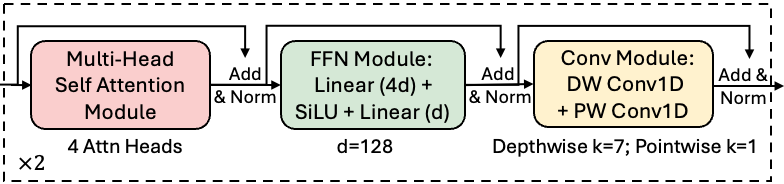
\includegraphics[width=0.9\textwidth]{Chapter_4/figures/p3.jpg}
\caption{Lightweight Conformer-like Transformer encoder used in the score-informed correction module.}
\label{fig:scoreinf_encoder}
\end{figure}

We use an embedding size of $d=128$, two encoder layers, and four attention heads.
A dropout rate of $0.1$ is applied after each sub-module.
Given the encoder outputs, a linear head predicts a scalar residual $\delta_i$ for each token.
The corrected velocity is then obtained by a bounded residual update:
\begin{equation}
\hat{V}^{\mathrm{corr}}_{t_i,p_i}
= \operatorname{clip}\!\Big(\hat{V}_{0,t_i,p_i} + \alpha\tanh(\delta_i),\, 0,\, 1\Big),
\label{eq:scoreinf:update}
\end{equation}
where $\alpha$ controls the maximum correction magnitude.
In all experiments, $\alpha=0.2$.
The corrected values replace the preliminary estimates at onset positions.
Non-onset entries remain unchanged.

The two correction modules reveal the main architectural contrast in this chapter.
The BiLSTM treats the task as dense frame-wise sequence correction.
The Transformer treats it as sparse onset-wise residual refinement.
Both use the same score source.
The later analysis shows that this difference in representation and inductive bias has a clear effect on generalization.

\subsection{Loss function}
\label{sec:scoreinf:loss}

All models are trained with the hybrid loss adopted in prior score-informed work~\cite{kim2024method}.
It combines frame-wise binary cross-entropy with onset-wise $\ell_1$ loss:
\begin{equation}
\mathcal{L}
= \frac{1}{|\mathcal{J}|}\sum_{(t,p)\in\mathcal{J}} \ell_{\mathrm{bce}}\big(V_{t,p},\hat{V}_{t,p}\big)
+ \frac{1}{|\mathcal{I}|}\sum_{(t,p)\in\mathcal{I}} \left|V_{t,p}-\hat{V}_{t,p}\right|.
\label{eq:scoreinf:loss}
\end{equation}
Here $\mathbf{V}$ is the ground-truth velocity target and $\hat{\mathbf{V}}$ is the predicted velocity output of either the baseline AMT branch or the score-informed system.
This hybrid supervision is useful because it constrains both the local onset value and the broader note sustain region, while still keeping note-level precision central to the objective.

\subsection{Post-Processing}
\label{sec:scoreinf:post}

MIDI velocity is defined at note onset. It reflects the instantaneous intensity of the keystroke rather than a time-varying loudness curve \cite{dan2006psy}. This onset-centered definition is also consistent with the physical mechanism of the piano: once a key has been fully depressed down, subsequent finger pressure does not further control the sounding intensity. Only specific string instruments such as the violin, where continuous loudness modulation is possible. The piano does not support this type of control, musically said, vibrato is impossible on the piano.

In our setting, a time-aligned MIDI score is available, which provides the note positions including onsets and duration (note frames). We therefore bypass AMT-style note detection and instead focus only on estimating the velocity value for each given note. During post-processing, the predicted velocity at the onset is taken and then assigned to the whole note event, consistent with the MIDI specification.

\section{Experimental Protocol}
\label{sec:scoreinf:exp}

The experiments are designed to answer four questions.
First, does the score-informed correction module improve a strong AMT baseline in-domain.
Second, how do the BiLSTM and Transformer correction designs differ in generalization behaviour.
Third, can the same correction principle be attached to several AMT backbones with only small overhead.
Fourth, how robust is the final score-informed design to moderate audio--score misalignment.

\subsection{Datasets}
\label{sec:scoreinf:datasets}

For training, we use the MAESTRO v3.0.0 dataset~\cite{hawthorne2019maestro} with its default train, validation, and test split.
MAESTRO contains 1,276 Yamaha Disklavier piano performances and more than 200 hours of precisely aligned audio--MIDI pairs.
The Disklavier setup is particularly valuable here because it provides high-fidelity note-level velocity targets together with realistic acoustic recordings.
For out-of-domain evaluation, we use the SMD dataset~\cite{smd}.
All models are trained only on the MAESTRO training split.
This deliberately strict protocol exposes cross-dataset behaviour clearly.

\subsection{AMT backbones and training setup}
\label{sec:scoreinf:training}

The chapter uses three representative velocity-enabled AMT backbones.
HPT~\cite{kong2021hpt} is adopted as the main testbed because it is lightweight and widely used.
HPPNet~\cite{wei2022hppnet} provides a parameter-efficient alternative.
DynEst~\cite{he2026dynest} provides a recent dynamics-oriented baseline.
For each selected model, we retrain its velocity branch as an audio-only baseline and compare it with a jointly trained counterpart that includes the proposed score-informed module.
For HPT, we evaluate both the BiLSTM and the Transformer correction designs.
For the broader cross-backbone comparison and robustness study, we use the Transformer design because it becomes the preferred final module after the generalization analysis.

Each model is trained for 120k iterations on a single NVIDIA RTX~3090 with 24~GiB memory.
We use Adam with a learning rate of $1\times10^{-4}$.
The learning rate is multiplied by $0.9$ every 10k iterations.
The batch size is 12.
The random seed is 86.
We select the best checkpoint by validation-set performance and then evaluate on the test sets.

\subsection{Evaluation metrics}
\label{sec:scoreinf:metrics}

We retain the note-level evaluation protocol introduced in Section~\ref{sec:velcomp:metrics} of Chapter~\ref{ch:velcomp}. 
Specifically, the present chapter reports three quantitative metrics on the denormalized MIDI velocity scale $[0,127]$: the mean absolute error (MAE), the standard deviation of the absolute error ($SD_{\mathrm{ae}}$), and Recall\textsubscript{10\%}. 
Their formal definitions follow exactly the notation and formulas given in Eqs.~\eqref{eq:velcomp_mae}, \eqref{eq:velcomp_sdae}, and \eqref{eq:velcomp_recall}. 
In this chapter, the evaluation set \(\mathcal{I}\) is onset-masked by the aligned score, so the comparison is carried out only at reference note positions. 
This yields a note-level evaluation and avoids the temporal bias of frame-wise scoring, where sustained notes would otherwise dominate the error.


A brief clarification is needed for the recall-style metric, because some earlier score-informed studies reported a different quantity under the name \emph{Recall} \cite{kim2024method}.
In those studies, the predicted velocity map was sparse, so the goal was simply to check whether the model produced a nonzero velocity value at the reference note position:
\begin{equation}
\mathrm{Recall}
= \frac{1}{|\mathcal{I}|}\sum_{i\in\mathcal{I}}
\mathbf{1}\!\left(\hat{V}_i > 0\right).
\label{eq:scoreinf:legacy_recall}
\end{equation}
This quantity measures note-position coverage rather than the accuracy of MIDI velocity itself. In our approach, and in most modern AMT baselines, the predicted velocity maps are dense as shown in Figure~\ref{fig:scoreinf_qualitative}. After post-processing, almost every aligned note onset therefore receives a nonzero estimated velocity, so the older Recall quickly saturates near \(100\%\) and becomes uninformative.

For this reason, the present chapter uses Recall\textsubscript{10\%}, following the same definition as Chapter~\ref{ch:velcomp}. 
This metric counts a note as correct only when the predicted velocity falls within a $10\%$ tolerance on the MIDI velocity scale. It is consistent with the velocity criterion used in the standard $NoteOn/OffwVelo$ evaluation implemented in the \texttt{mir\_eval} package \cite{raffel2014mireval}, which is widely used in music transcription research. Using this convention makes the evaluation easier to reproduce and helps maintain comparability with established AMT benchmarks.

\section{Results and Analysis}
\label{sec:scoreinf:results}

\subsection{Validation on the score-informed correction}
\label{sec:scoreinf:results:maestro}

We first attach the proposed modules to HPT and denote the resulting systems as Score-HPT.
HPT is used as the initial testbed because it is lightweight and prevalent in recent piano transcription work.
This lets us isolate the effect of score-informed correction before extending the method to other backbones.
Table~\ref{tab:scoreinf_maestro} summarizes the results on the MAESTRO test set.

\begin{table}[h]
    \centering
    \setlength{\tabcolsep}{6pt}
    \begin{tabular}{l|cccc}
    \toprule
    \multicolumn{1}{c|}{\multirow{2}{*}{\textbf{Model \& Inputs}}}
      & \multicolumn{4}{c}{\textbf{MAESTRO test set}} \\
    \cmidrule(l){2-5}
      & MAE $\downarrow$ & SD\textsubscript{ae} $\downarrow$ & Recall$_{10\%}$ $\uparrow$ & \# Params \\
    \midrule
    \textbf{HPT} & & & & \\
    audio & 4.6 & 6.1 & 80.6\% & 4.1M \\
    \midrule
    \textbf{Score-HPT (BiLSTM applied)} & & & & \\
    audio + onset & 4.2 & 5.2 & 88.2\% & 5.8M \\
    audio + onset + frame & 3.6 & 4.5 & 95.6\% & 7.5M \\
    audio + onset + frame$_{\text{ex}}$ & 3.5 & 4.5 & 95.8\% & 7.5M \\
    \midrule
    \textbf{Score-HPT (Transformer applied)} & & & & \\
    audio + onset & 4.0 & 4.8 & 93.8\% & 5.0M \\
    audio + onset + frame & 4.0 & 4.7 & 93.9\% & 5.0M \\
    audio + onset + frame$_{\text{ex}}$ & 3.9 & 4.7 & 94.0\% & 5.0M \\
    \bottomrule
    \end{tabular}
    \caption{Comparison of HPT and Score-HPT on the MAESTRO test set. Lower values are better for MAE and \(SD_{\mathrm{ae}}\), while higher values are better for Recall$_{10\%}$.}
    \label{tab:scoreinf_maestro}
\end{table}

Two observations matter here.
First, both correction modules consistently improve the audio-only HPT baseline.
This confirms that aligned score information is useful even when inserted only after the AMT velocity branch.
Second, the BiLSTM achieves the strongest in-domain fit on MAESTRO, especially with onset $+$ frame$_{\text{ex}}$.
This shows that dense frame-wise recurrent correction is expressive enough to model the task very closely.
However, the later generalization analysis will show that the strongest in-domain fit is not the same as the best final design.
The Transformer reaches slightly higher MAE on MAESTRO, but it does so with fewer parameters and with a correction mechanism that is easier to transfer across backbones.

\begin{figure}[t]
\centering
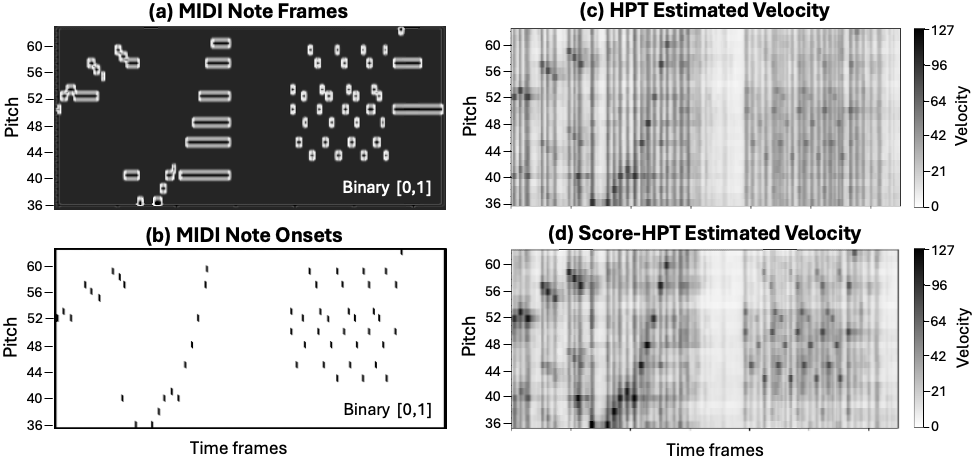
\includegraphics[width=\textwidth]{Chapter_4/figures/p4thesis.jpg}
\caption{Qualitative comparison between HPT and Score-HPT (Transformer applied). The refined estimate is more concentrated around onset locations while remaining fully populated.}
\label{fig:scoreinf_qualitative}
\end{figure}

Figure~\ref{fig:scoreinf_qualitative} gives a qualitative view of this effect.
Compared with the baseline, Score-HPT produces a cleaner onset-centered velocity pattern.
This is consistent with the intended role of MIDI velocity as an onset attribute.
The score-informed module does not remove the dense map predicted by the AMT branch.
Instead, it reshapes the estimate so that the onset locations become more informative.

\subsection{Cross-dataset generalization}
\label{sec:scoreinf:results:generalization}

To study generalization, we track learning curves on the MAESTRO validation set and on a held-out 10\% subset of SMD, which does not provide an official validation split.
Figures~\ref{fig:scoreinf_learning_bilstm_transformer} show that all score-informed HPT variants outperform the plain HPT baseline on both in-domain and out-of-domain data.
For the Transformer family, the onset $+$ frame condition gives the strongest overall cross-dataset behaviour, although the difference between score feature variants remains modest.

\begin{figure}[h!]
\centering
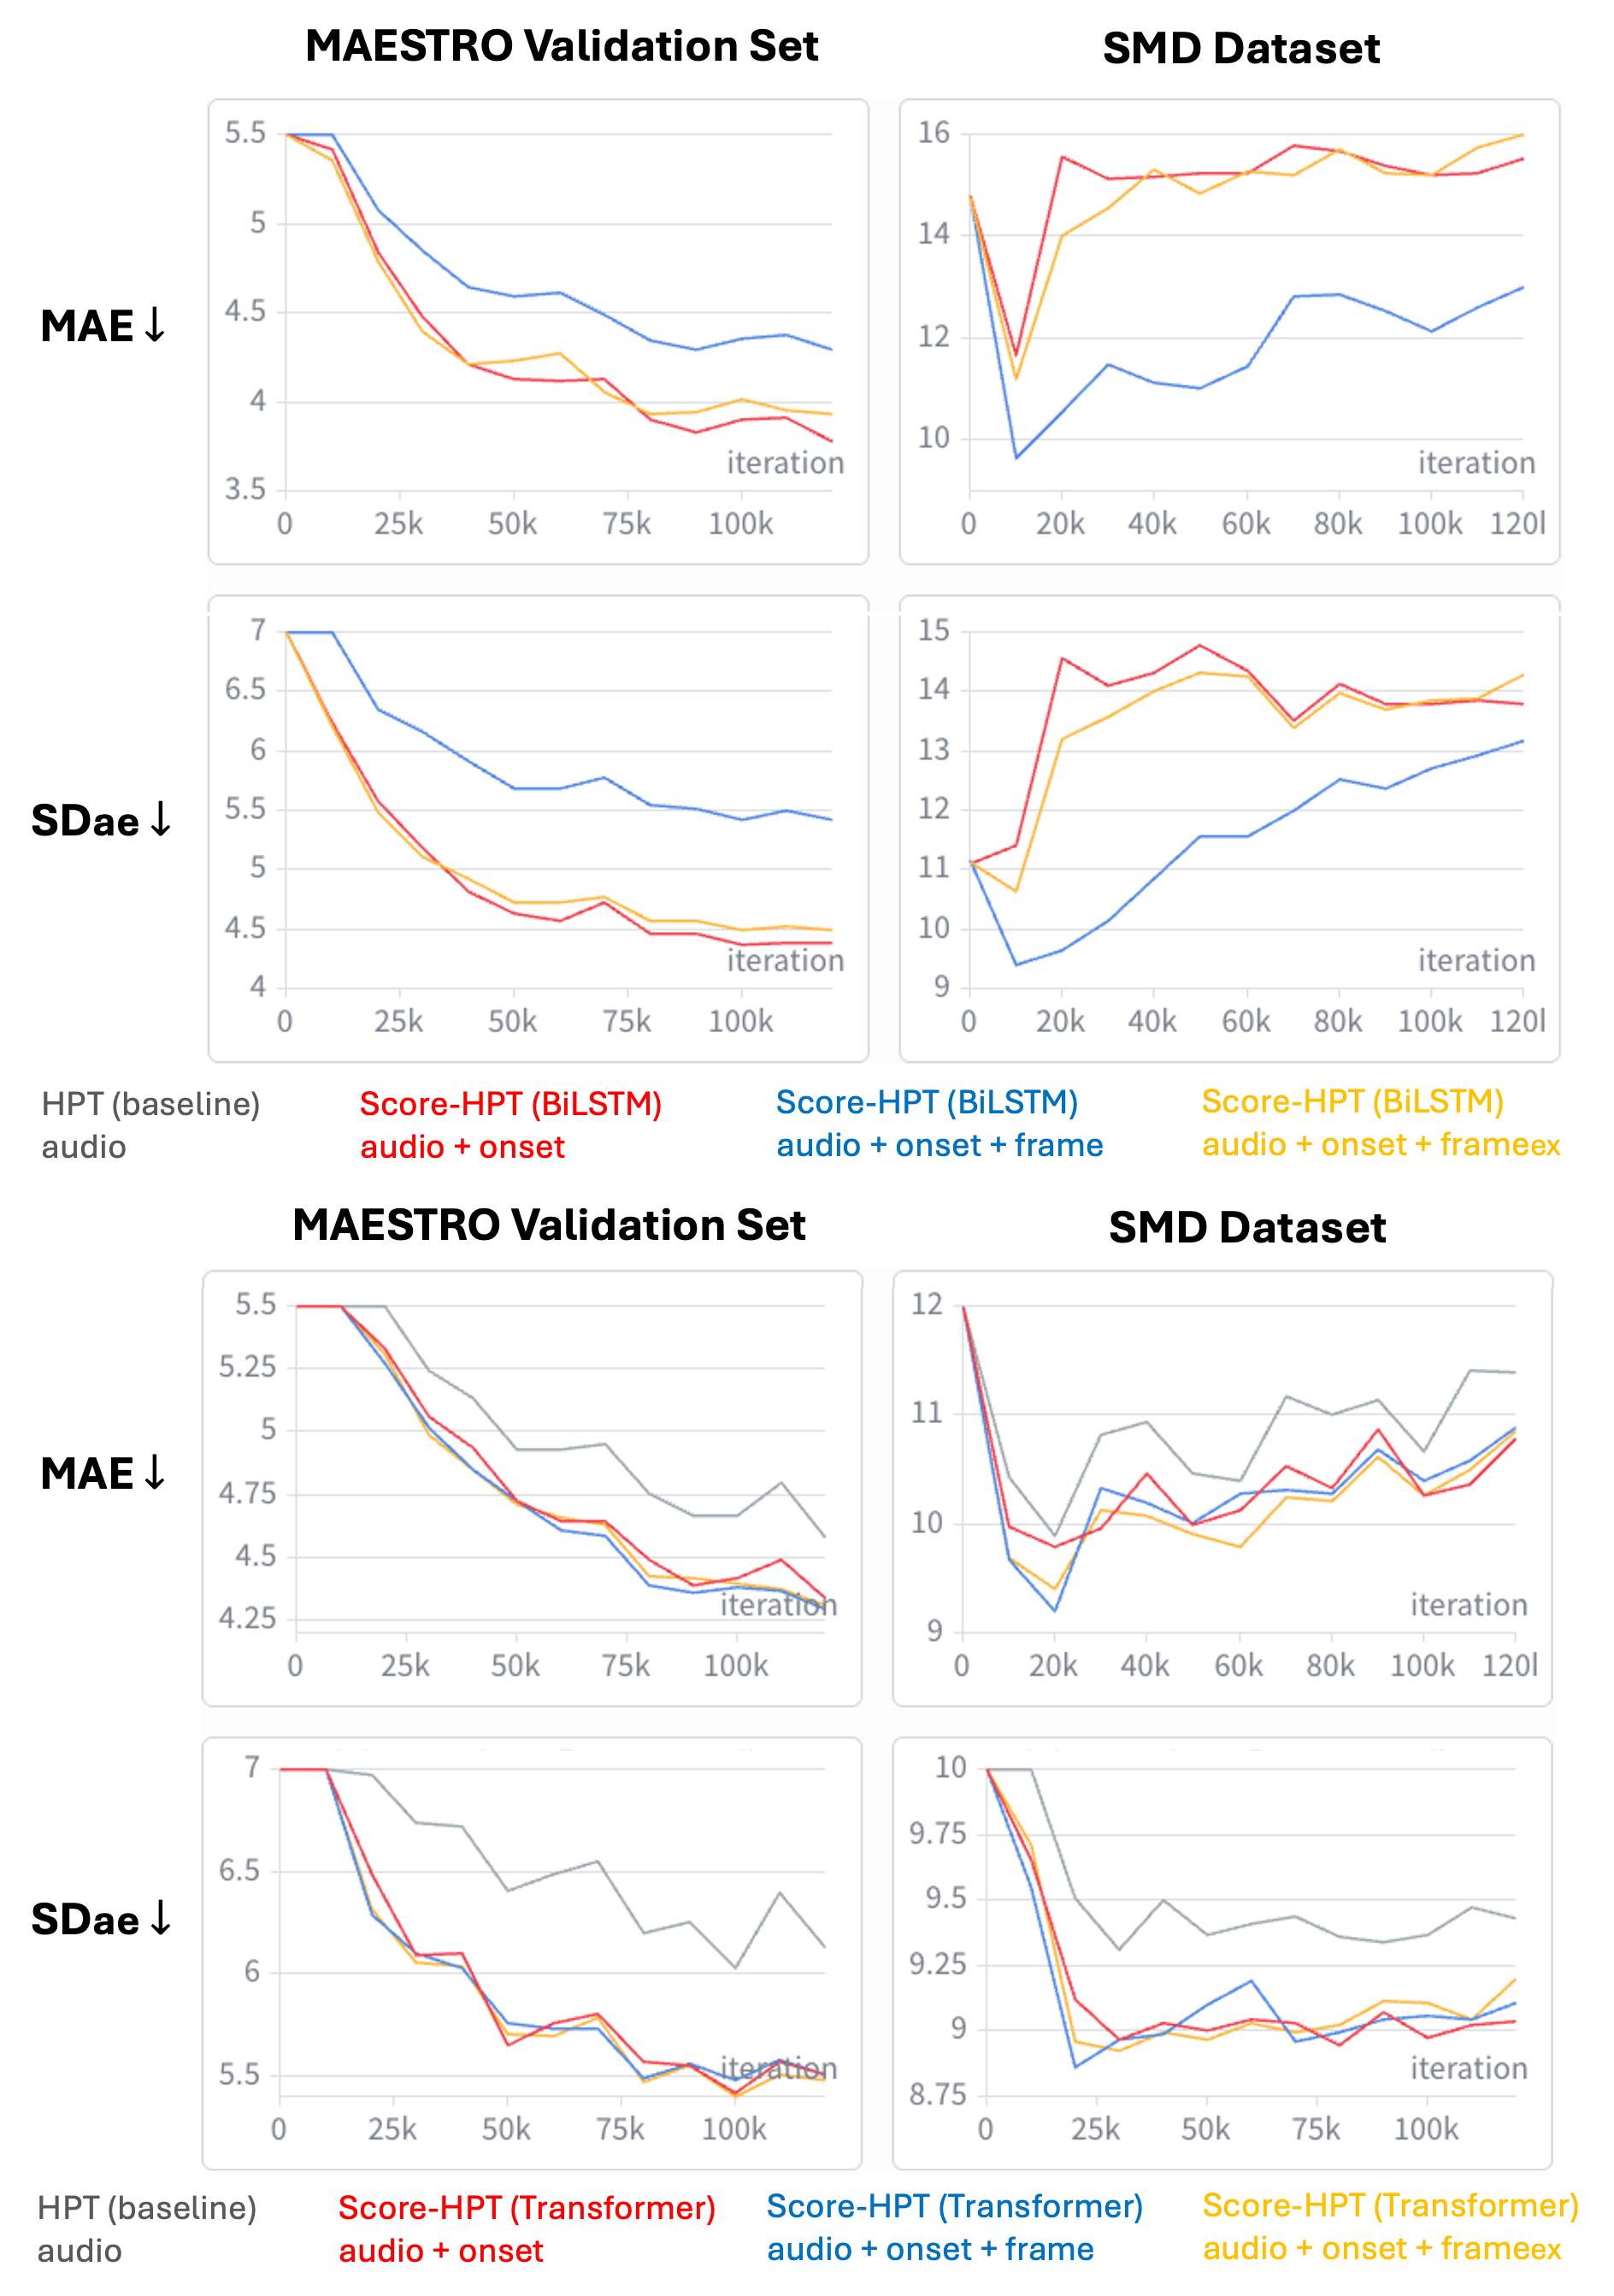
\includegraphics[width=0.96\textwidth]{Chapter_4/figures/p5thesis.png}
\caption{Learning curves for HPT and Score-HPT variants using the BiLSTM and Transformer correction module. All models are trained on the MAESTRO training split and evaluated every 10k iterations.}
\label{fig:scoreinf_learning_bilstm_transformer}
\end{figure}

A clear pattern appears during training.
Performance on MAESTRO improves steadily.
Performance on SMD peaks earlier and then degrades.
This indicates that prolonged training overfits to MAESTRO-specific acoustics.
Similar sound biases in AMT velocity estimation were also reported in \cite{martak2026soundmusicbias}.
The score-informed module does not remove this problem completely.
However, it shifts the error curves downward and stabilizes out-of-domain behaviour.
This supports the view that the aligned score acts as an acoustics-invariant structural prior.

The contrast between the BiLSTM and the Transformer is especially informative.
The BiLSTM tends to fit MAESTRO more aggressively, but its out-of-domain degradation is also more pronounced.
This behaviour is consistent with the way the two modules process the sequence.
The BiLSTM consumes all 1001 frames, including many highly redundant sustain frames.
Adjacent frames often carry very similar acoustic-envelope information.
A recurrent model can therefore reduce training loss by memorizing dataset-specific loudness trajectories, microphone responses, and reverberation patterns that repeat within MAESTRO recordings.
Its bidirectional hidden state also entangles each correction with broad frame-level acoustic context.
That context is helpful in-domain, but it is also where room and recording biases reside.
The BiLSTM variant is additionally larger than the Transformer variant, which further increases its capacity to absorb these biases.

The Transformer has a different inductive bias.
It operates only on onset tokens rather than on the full frame lattice.
This removes most of the redundant sustain frames that are easiest to overfit.
Self-attention then models note-to-note relations directly on the symbolic event sequence, while the bounded residual update in Eq.~\eqref{eq:scoreinf:update} constrains the magnitude of each correction.
In effect, the Transformer is encouraged to learn \emph{where} and \emph{how much} the preliminary velocity should be adjusted, instead of re-modelling the full acoustic envelope.
This yields a slightly less aggressive in-domain fit than the BiLSTM, but better cross-dataset stability.
For this reason, the Transformer becomes the main correction module in the remainder of the chapter.

\subsection{Comparison with existing systems}
\label{sec:scoreinf:results:comparison}

We next compare the Transformer-based correction strategy with existing score-informed systems and representative AMT models on the SMD dataset.
To keep the comparison fair, all models follow the same training protocol and use only the MAESTRO training split for learning.
Following the generalization analysis above, we use onset $+$ frame for all proposed Transformer-based variants.
Table~\ref{tab:scoreinf_smd} summarizes the results. Specifically, Recall$_{10\%}$ results of hFT-Transformer and Transkun v2 are obtained from the MIREX2024: Polyphonic Transcription challenge.\footnote{\url{https://music-ir.org/mirex/wiki/2024:Polyphonic_Transcription_Results}}

\begin{table}[b]
    \centering
    \setlength{\tabcolsep}{4pt}
    \small
    \begin{tabular}{l|rrrr}
    \toprule
    \multicolumn{1}{c|}{\multirow{2}{*}{\textbf{Model}}}
      & \multicolumn{4}{c}{\textbf{SMD dataset}} \\
    \cmidrule(l){2-5}
      & MAE $\downarrow$ & SD\textsubscript{ae} $\downarrow$ & Recall$_{10\%}$ $\uparrow$ & \# Params \\
    \midrule
    \textbf{Score-informed methods} & & & & \\
    DiffVel~\cite{kim2023diffvel} & 19.7 & 13.1 & -- & -- \\
    FiLM Conv~\cite{kim2023score} & 15.1 & 12.3 & -- & -- \\
    FiLM U-Net~\cite{kim2024method} & 9.9 & 7.8 & 73.0\%\tablefootnote{The reported 89.7\% in their paper is standard Recall, a less strict metric than our Recall$_{10\%}$.} & 8.8M \\
    \midrule
    \textbf{Proposed (Transformer applied)} & & & & \\
    Score-HPT & \textbf{8.0} & \textbf{6.9} & 80.3\% & 5.0M \\
    Score-HPPNet & 9.2 & 7.3 & 79.3\% & 1.5M \\
    Score-DynEst & \textbf{8.0} & \textbf{6.9} & 77.6\% & 14.3M \\
    \midrule
    \textbf{AMT systems} & & & & \\
    HPT~\cite{kong2021hpt} & 10.0 & 8.8 & 62.5\% & 4.1M \\
    HPPNet (no CQT)~\cite{wei2022hppnet} & 10.6 & 9.0 & 60.2\% & 0.5M \\
    DynEst (no BSSL)~\cite{he2026dynest} & 10.4 & 8.8 & 59.6\% & 13.3M \\
    hFT-Transformer~\cite{toyama2023hft} & 9.9 & 7.3 & 76.5\% & 5.5M \\
    Transkun v2~\cite{yan2024semicrf} & 13.3 & 11.9 & \textbf{82.1\%} & 13.6M \\
    \bottomrule
    \end{tabular}
    \caption{Comparison on the SMD dataset. All models are trained only on the MAESTRO training split.}
    \label{tab:scoreinf_smd}
\end{table}

Table~\ref{tab:scoreinf_smd} shows that Score-HPT and Score-DynEst achieve the best MAE and \(SD_{\mathrm{ae}}\) under this protocol.
They outperform dedicated score-informed FiLM models as well as several strong velocity-enabled AMT systems.
The result is notable because the added correction module is small.
The parameter overhead is about 1M.

The same correction principle is also effective beyond HPT.
When attached to HPPNet and DynEst, it again improves the corresponding baseline.
This supports the main thesis claim of the chapter.
The benefit does not depend on one transcription backbone.
Instead, the method behaves as a reusable refinement layer.
Even when HPPNet and DynEst are retrained with log-Mel spectrograms rather than with their original CQT or Bark-scale specific loudness inputs, the score-informed module still yields a consistent gain.
This strengthens the argument that the correction principle itself is robust.

One further detail is worth noting.
Although Transkun v2 defines a very strong state of the art in note transcription, it is less competitive in velocity MAE and \(SD_{\mathrm{ae}}\).
A plausible reason is that its core SemiCRF design is primarily optimized for note-event modelling rather than for precise dynamics regression.
This observation reinforces the main claim of the chapter: strong note transcription does not automatically imply strong note-level velocity estimation.
A dedicated but lightweight correction layer can still add value.

\subsection{Robustness to audio--score misalignment}
\label{sec:scoreinf:results:robustness}

The previous thesis draft treated score alignment quality mainly as a limitation.
The updated SMC 2026 paper allows this question to be tested directly.
To evaluate robustness under imperfect synchronization, we conduct timing-shift experiments using artificial score displacements from $\pm0.1$ to $\pm2.5$ seconds, following \cite{kim2024method}.
These shifts are applied to the SMD evaluation data.
For example, a $+0.1$ shift means that the original aligned score is intentionally delayed by 0.1 seconds.
All models evaluated here are the same final models used in the cross-backbone comparison above.
They are trained only on perfectly aligned MAESTRO data.
The results are summarized in Figure~\ref{fig:scoreinf_robustness}.

\begin{figure}[t]
\centering
% Assumes the robustness figure from the updated paper is stored in the chapter figure directory.
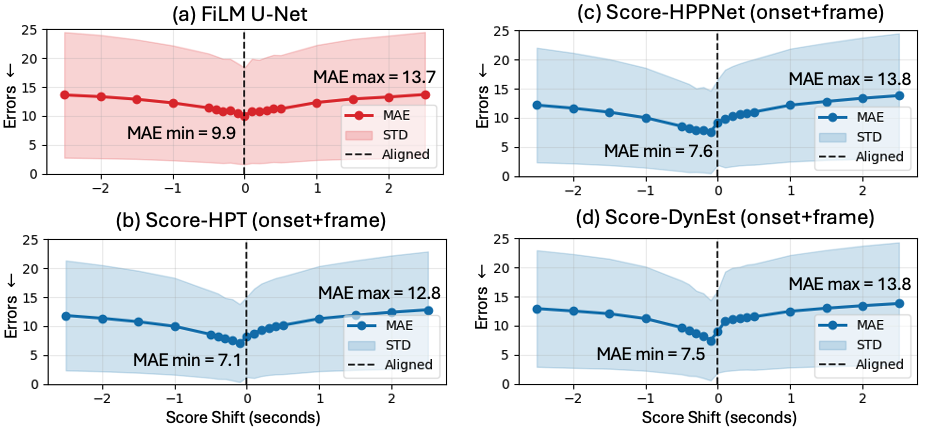
\includegraphics[width=\textwidth]{Chapter_4/figures/p6thesis.jpg}
\caption{Robustness evaluation on data derived from the SMD dataset, using audio--score misalignments of $\pm$0.1, 0.2, 0.3, 0.4, 0.5, 1, 1.5, 2, and 2.5 s.}
\label{fig:scoreinf_robustness}
\end{figure}

A methodological point is important here.
In the earlier benchmark of \cite{kim2024method}, shifted scores were used as model inputs but the original unshifted score was still used during post-processing.
That choice follows the earlier evaluation tradition of \cite{kim2023score}, but it introduces a temporal inconsistency.
If a model is conditioned on a shifted score, then its output is tied to that shifted note grid.
Post-processing should therefore use the same shifted score.
We adopt this internally consistent protocol in the present chapter.
Under this refinement, FiLM U-Net is substantially more robust than originally implied by the earlier report.

Applying this refined protocol, Score-HPT achieves the strongest robustness curve on SMD.
More broadly, all score-informed methods degrade only moderately relative to the perfectly aligned case.
Given that MIDI velocity spans the range 0 to 127, the observed increase of only a few units in MAE or \(SD_{\mathrm{ae}}\) under even large global shifts remains small in absolute terms.
Minor shifts can even lead to slight improvements for some proposed variants.
A plausible interpretation is that the AMT branch already produces temporally fuzzy onset-wise velocity estimates, and a small score displacement may occasionally compensate for that fuzziness.
The important conclusion is not that alignment no longer matters.
Rather, it is that the proposed late-correction design is surprisingly tolerant to moderate global timing mismatch.
This makes the method more realistic for educational and archival use, where score synchronization is often good but not perfect.

\section{Discussion}
\label{sec:scoreinf:discussion}

The main finding of this chapter is that score information is most useful when it is treated as a structural prior rather than as a full replacement for the acoustic model.
The AMT backbone still supplies the initial estimate of performance intensity.
The score-informed module only performs a targeted correction at onset locations.
This division of labour keeps the system lightweight and explains why the gain transfers across backbones.
It also clarifies why score information helps cross-dataset behaviour.
The score does not change with microphone placement, room acoustics, or recording chain.
It regularizes a prediction target that is otherwise acoustically fragile.

The retained BiLSTM experiment makes this point sharper.
The BiLSTM results show that score-informed correction is not inherently tied to attention.
A recurrent module can also exploit score support and can even fit the training domain more strongly.
However, the Transformer is a better final design because its inductive bias matches the task more closely.
Velocity is a note-onset attribute.
The onset-token Transformer models note events directly.
The BiLSTM instead processes a long dense frame sequence in which many frames correspond to sustain and acoustic decay rather than to distinct note decisions.
This is precisely where overfitting to recording-specific envelopes becomes easier.
The Transformer therefore trades a small amount of in-domain fit for better portability and generalization.

The robustness experiments also refine the chapter's earlier interpretation of the alignment assumption.
The system is clearly not immune to arbitrary score error.
The present test perturbs the score with a \emph{global} shift.
That is only one form of alignment imperfection.
Harder failures remain possible when ornaments are missing, repeated sections are mismatched, local tempo warping is severe, or the score itself omits performed notes.
Still, the robustness result is important because it shows that moderate timing offsets do not immediately destroy the value of late correction.
The practical bottleneck is therefore narrower than a strict perfect-alignment assumption might suggest.

From a thesis perspective, this chapter complements Chapter~\ref{ch:velcomp} in an important way.
Chapter~\ref{ch:velcomp} showed that velocity can be completed from symbolic structure alone.
The present chapter shows that, when audio and score are both available, a modular score-informed correction layer can outperform both audio-only AMT baselines and dedicated score-informed fusion models.
The chapter also provides a bridge to Chapter~\ref{ch:audiodyn}.
Here the score is still assumed to define note events.
The next chapter will relax that focus and move toward broader dynamic descriptors that are not reducible to note-level velocity alone.

\section{Chapter Summary and Outlook}
\label{sec:scoreinf:conclusion}

This chapter presented a modular score-informed correction framework for refining MIDI velocity in automatic piano transcription when a reference score is available.
The core idea is to keep the AMT backbone unchanged and to use score information only as a late residual correction signal.
Experiments on MAESTRO and SMD show that this simple principle is effective.
The score-informed module improves a strong AMT baseline in-domain, improves cross-dataset behaviour, transfers across several AMT backbones, and remains robust to moderate global audio--score misalignment.

The retained BiLSTM analysis adds an important thesis insight.
A stronger in-domain fit does not necessarily imply a better final architecture.
Because the BiLSTM processes dense frame sequences and carries broad acoustic context through recurrent hidden states, it is more prone to absorbing domain-specific envelope patterns.
The onset-token Transformer is therefore preferred because it aligns better with the note-level correction objective and generalizes more reliably.

The most immediate next step is to test more realistic alignment errors than uniform global shifts.
Local warping, missing ornaments, structural repeats, and partially incorrect score content are likely to be harder than the robustness settings studied here.
A second direction is transfer beyond piano.
The current evaluation remains piano-specific because reliable note-level velocity ground truth is rare for other instruments.
Extending the correction principle to broader instrumental settings will likely require weaker supervision, transfer learning, or self-supervised pretraining.
These directions connect directly to the broader thesis agenda on expressive data recovery under imperfect supervision.

% Retain per-chapter bibliography if the thesis build uses chapter-wise references.
% Remove the next line if the main thesis file uses a single global bibliography.
% \bibliography{smc2026}
